\section{Organización del proyecto}
\label{organiz}

Para incentivar el trabajo en paralelo en proyecto, se han creado diferentes grupos de trabajo identificados por las tareas que conllevan:

\begin{figure}[h]
	\centering 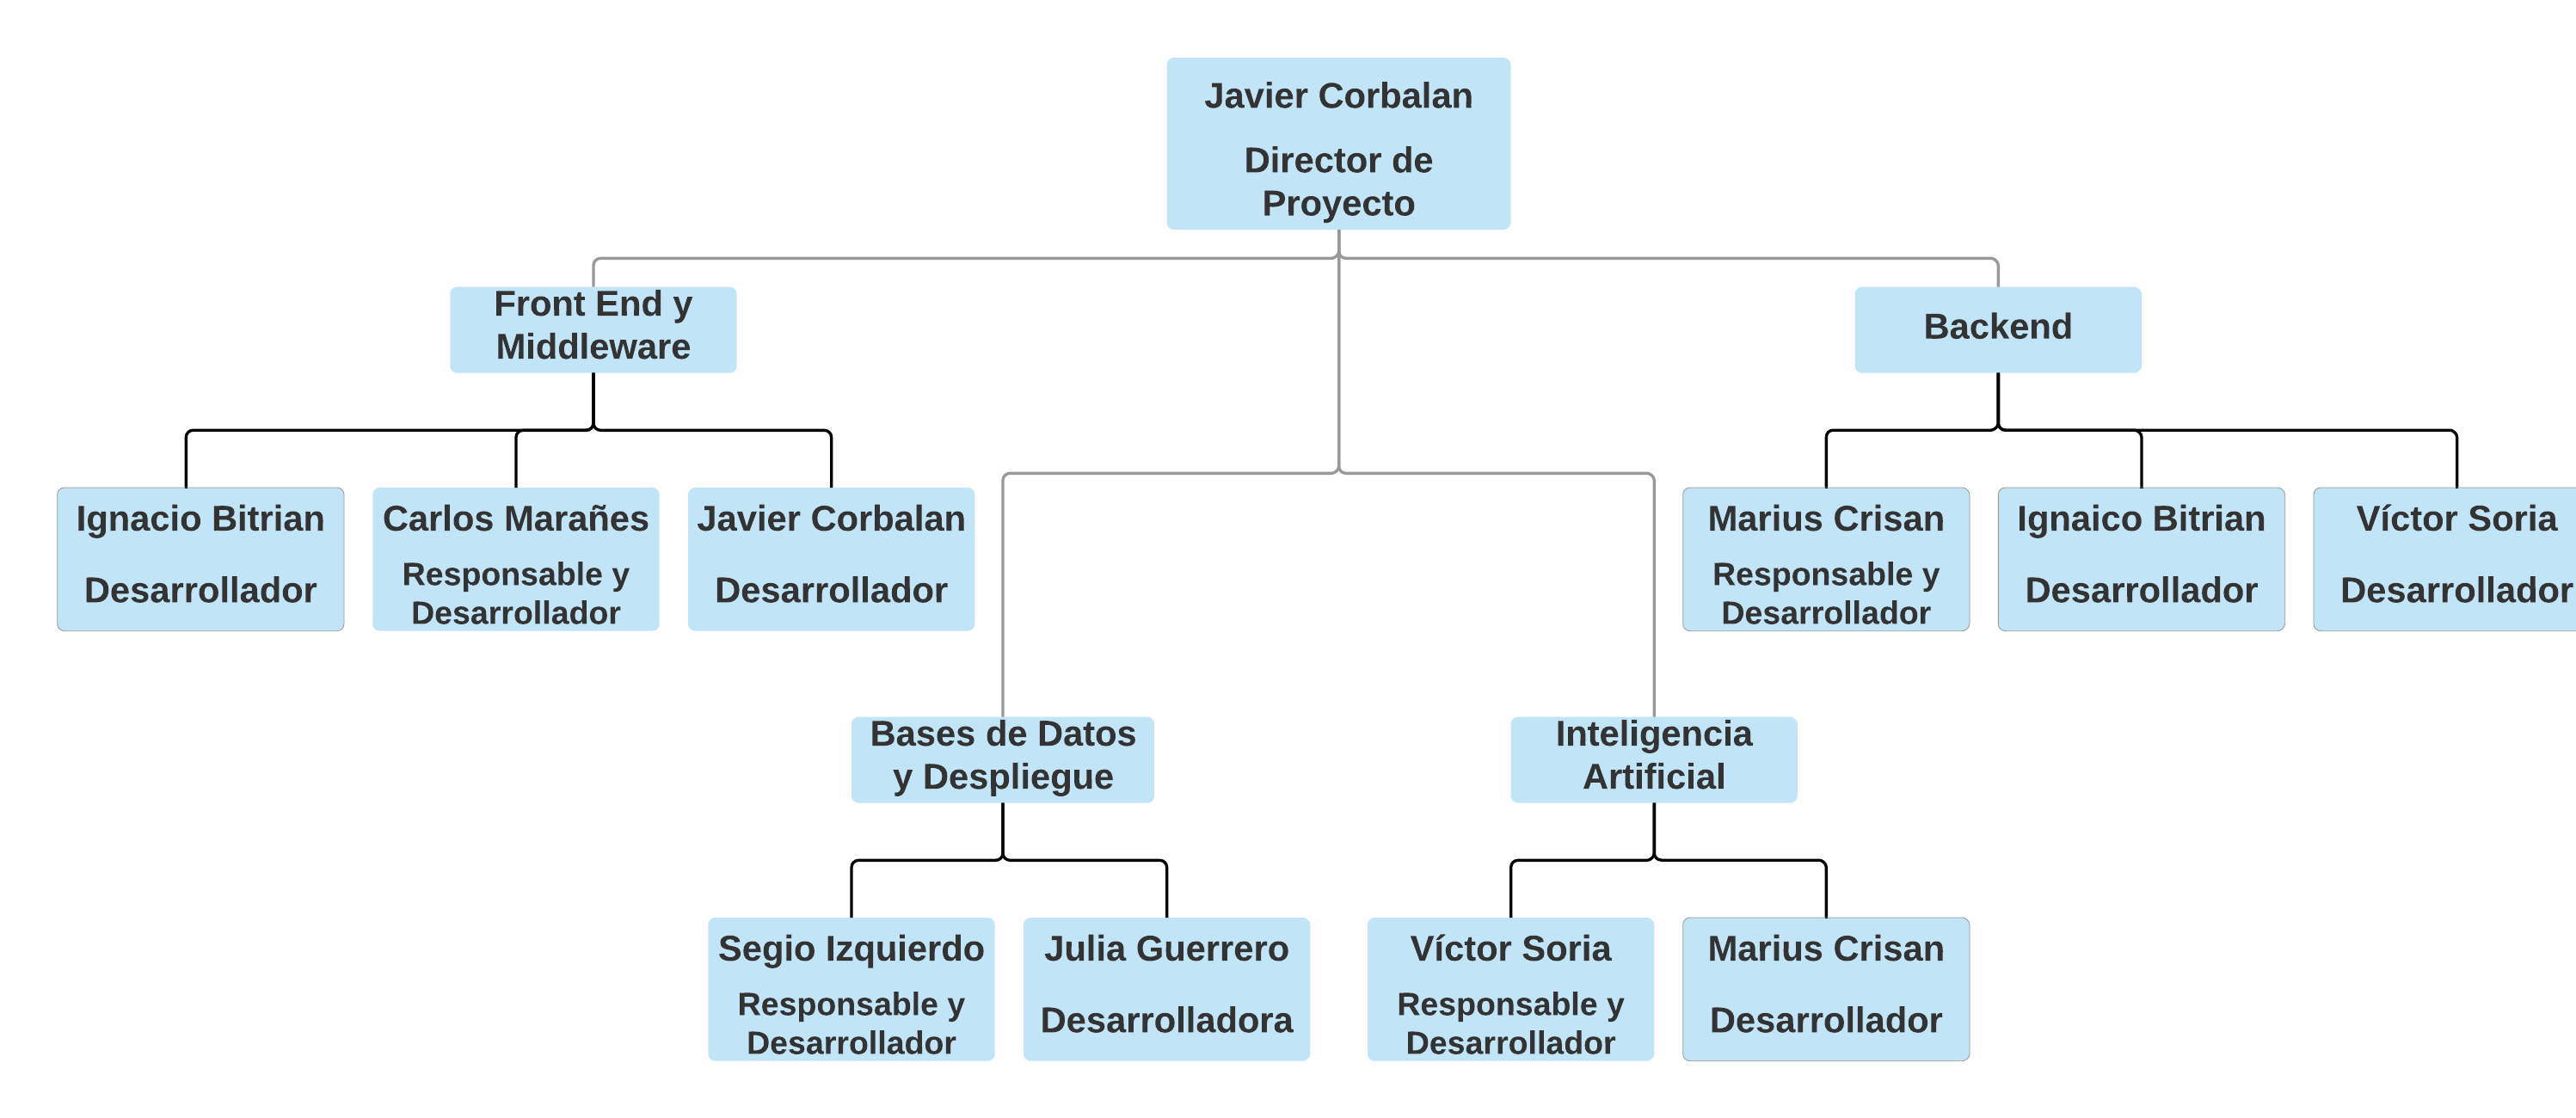
\includegraphics[scale=0.6]{figuras/organigrama.png}
\end{figure}

\begin{enumerate}
\item Desarrollo del Frontend y Middleware: Incluye el desarrollo de la interfaz y las vistas de la aplicación, además de la gestión de la comunicación entre los jugadores y servidor durante el desarrollo la partida.
\item Despliegue e implementación de la base de datos: Incluye el análisis y diseño de la base de datos, la capa de acceso a datos, despliegue de la aplicación y mantenimiento.
\item Desarrollo de la inteligencia artificial: Incluye el análisis del juego, diseño e implementación de un agente de inteligencia artificial.
\item Desarrollo del Backend: Implementación de los servicios web, tratamiento de peticiones, generación de páginas dinámicas (servlets) y la lógica del juego.
\end{enumerate}

La elección del director se ha llevado a cabo a través de una votación de mayoría simple.
